% \chapter{Drawings - Robot end effector}\label{cha:endeffector}
% \begin{figure}[h]
%     \centering
%     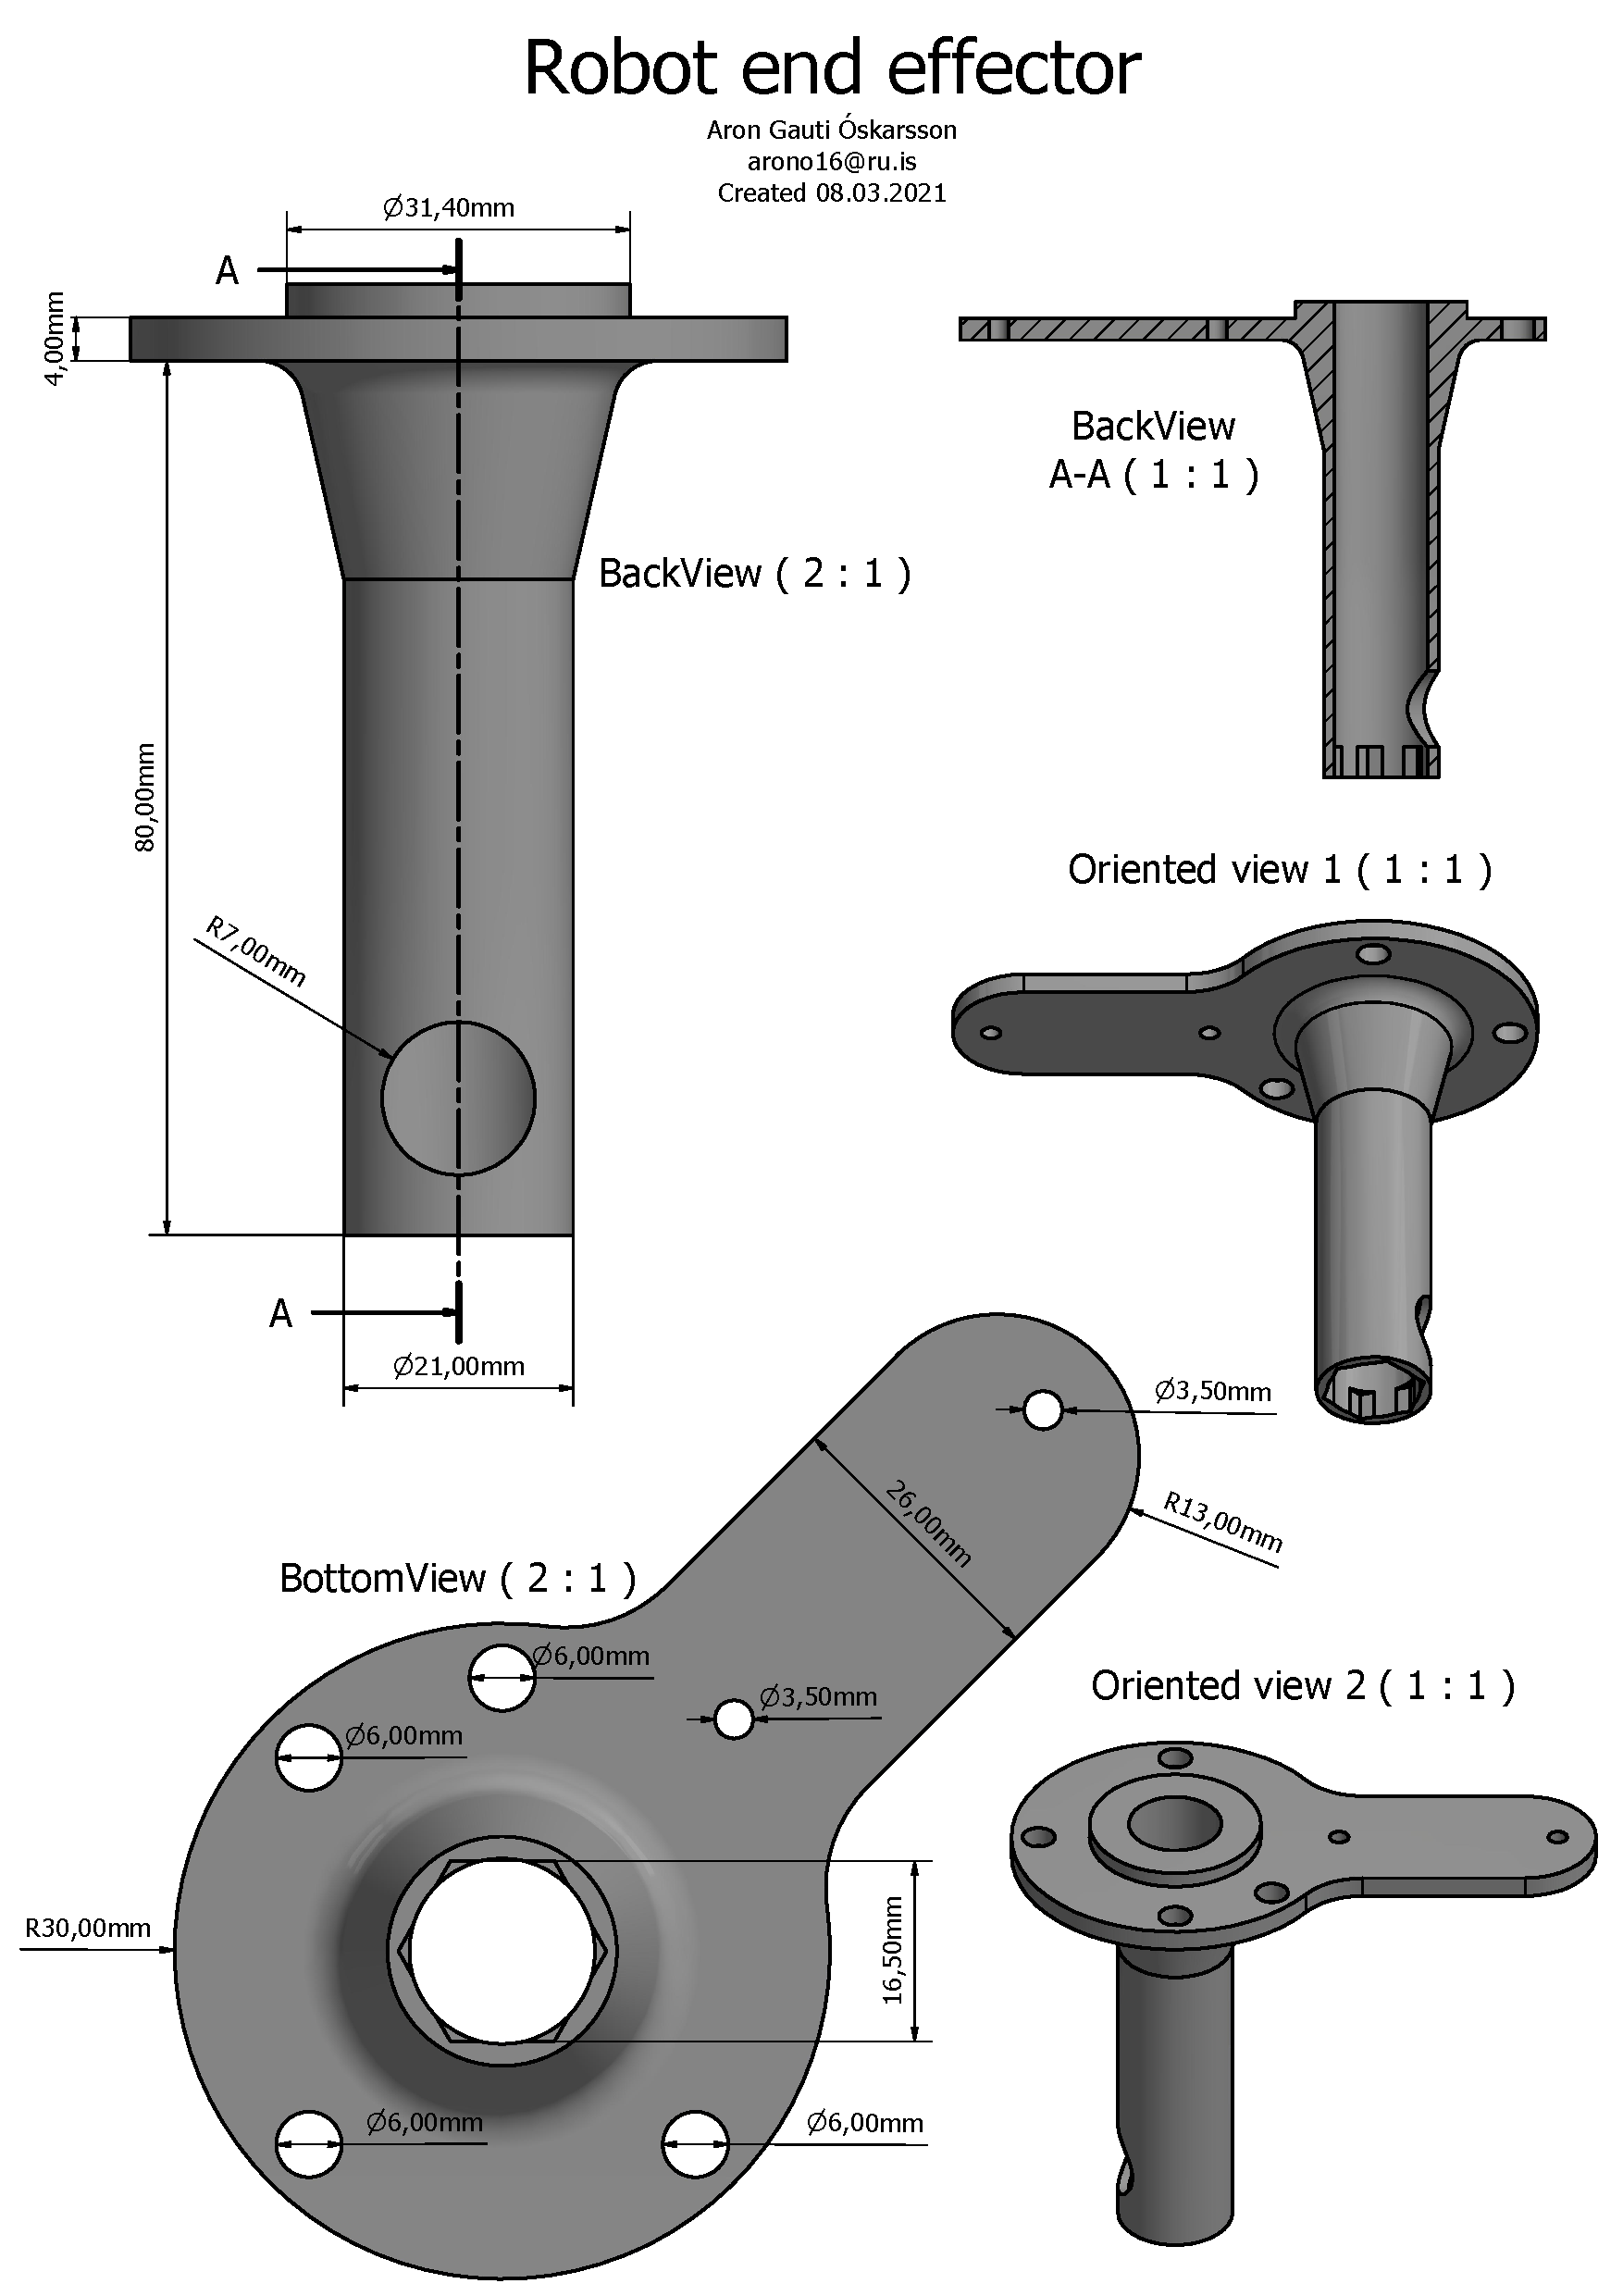
\includegraphics[width=0.7\textwidth]{graphics/model_panda_vacuumnewportrait.pdf}
%     \caption{Robot end effector}
%     \label{fig:my_label}
% \end{figure}
%Hægt að vera með tvær týpur sýnist þessi fyrir neðan betri

\definecolor{gray}{rgb}{0.4,0.4,0.4}
\definecolor{darkblue}{rgb}{0.0,0.0,0.6}
\definecolor{cyan}{rgb}{0.0,0.6,0.6}

\lstset{
  basicstyle=\ttfamily,
  columns=fullflexible,
  showstringspaces=false,
  commentstyle=\color{gray}\upshape
}

\lstdefinelanguage{XML}
{
  morestring=[b]",
  morestring=[s]{>}{<},
  morecomment=[s]{<?}{?>},
  stringstyle=\color{black},
  identifierstyle=\color{darkblue},
  keywordstyle=\color{cyan},
  morekeywords={xmlns,version,type}% list your attributes here
}
\appendix

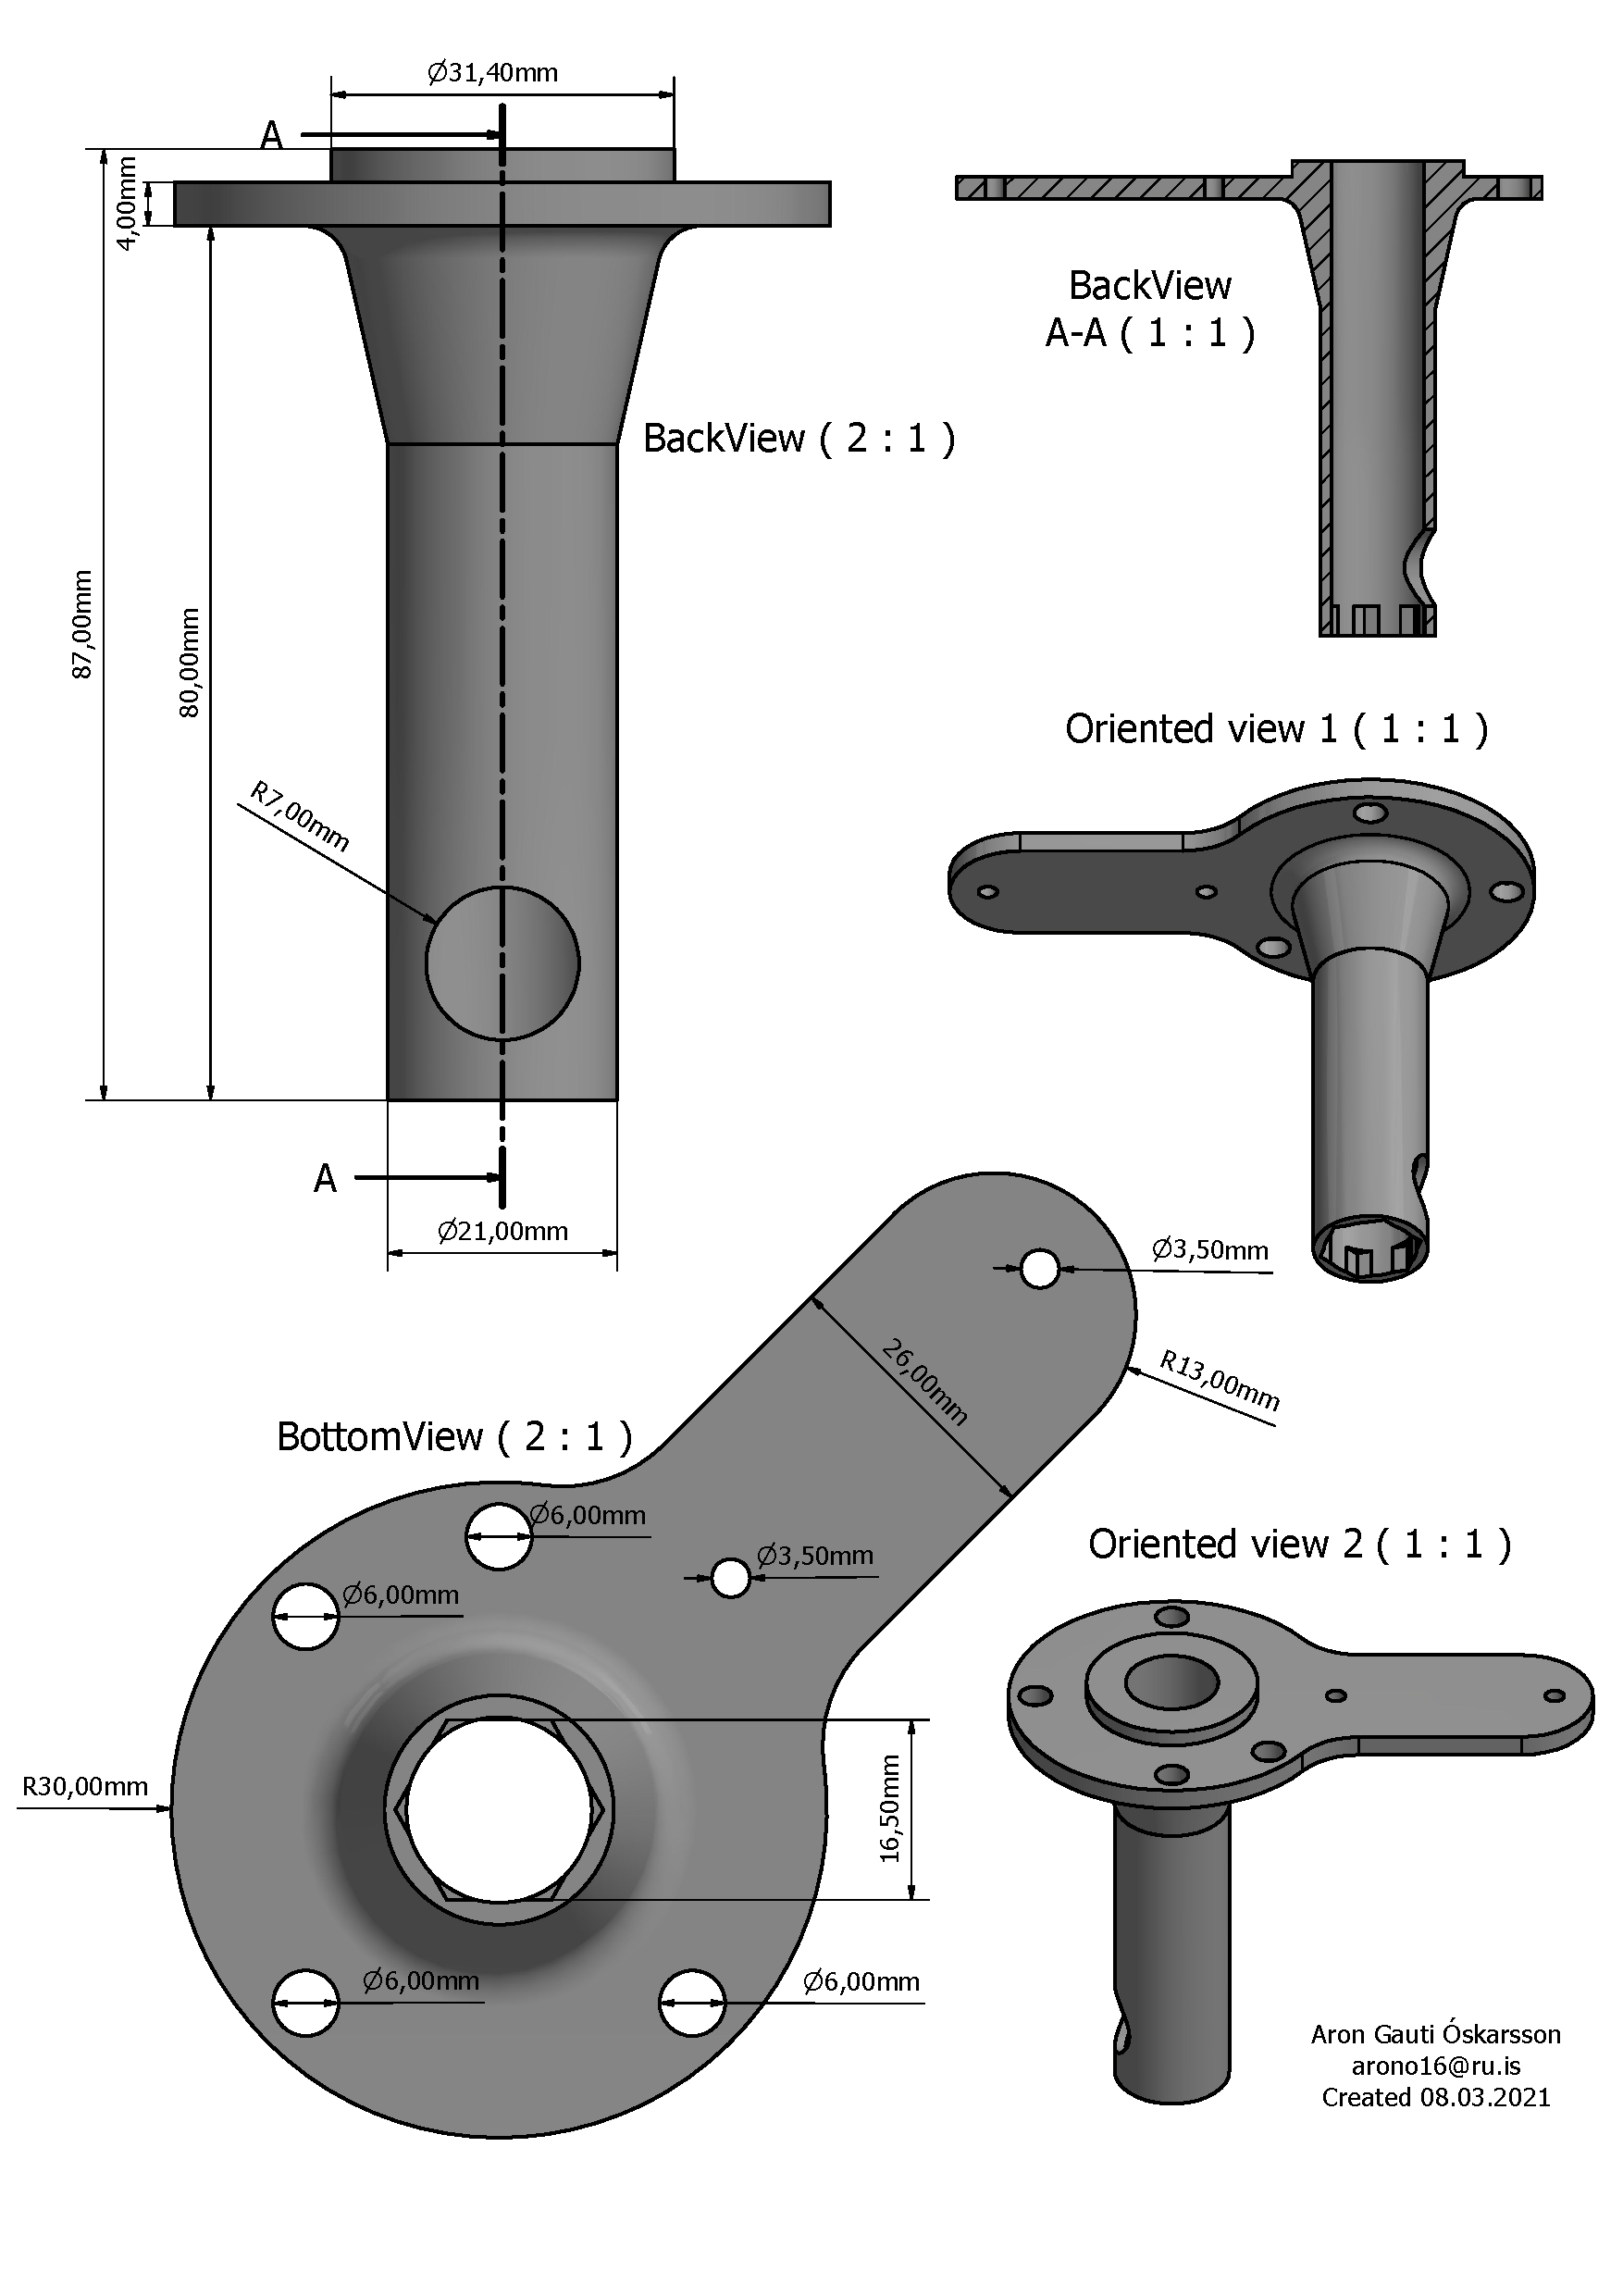
\includepdf[scale=0.7,pages=1,pagecommand=\chapter{Drawings - Robot end effector}\label{cha:endeffector}, offset=0 -4cm]{graphics/suctionDrawing.pdf}

\chapter{Code}  \label{app:code}
The code is also on Github link: \url{https://github.com/arongauti/MSc-projectAGO}
\section{pick-and-place.py}\label{sec:pickandplace}
\lstinputlisting[language=Python]{appendix/codes/pick_and_place.py}
\pagebreak

\section{v2pick-and-place.py}\label{sec:v2pickandplace}
\lstinputlisting[language=Python]{appendix/codes/v2pick_and_place.py}
\pagebreak

\section{find-pickpoint.py}\label{sec:findpickpoint}
\lstinputlisting[language=Python]{appendix/codes/find_pickpoint3.py}
\pagebreak

\section{v2find-pickpoint.py}\label{sec:v2findpickpoint}
\lstinputlisting[language=Python]{appendix/codes/v2find_pickpoint.py}
\pagebreak

\section{difference.py}\label{sec:difference}
\lstinputlisting[language=Python]{appendix/codes/difference.py}
\pagebreak

\section{v2difference.py}\label{sec:v2difference}
\lstinputlisting[language=Python]{appendix/codes/v2difference.py}
\pagebreak

\section{panda-bringup.launch}\label{sec:pandabringup}
\lstinputlisting[language=XML]{appendix/panda_bringup.launch}
\pagebreak
\section{Config file yolo-obj\_new.cfg}\label{sec:config}
\lstinputlisting[]{appendix/codes/yolo-obj_new.cfg}
\pagebreak

\chapter{Matlab results}
\section{Results on known items}\label{sec:apIoUresults}
\begin{figure}[h]
 \centering 
 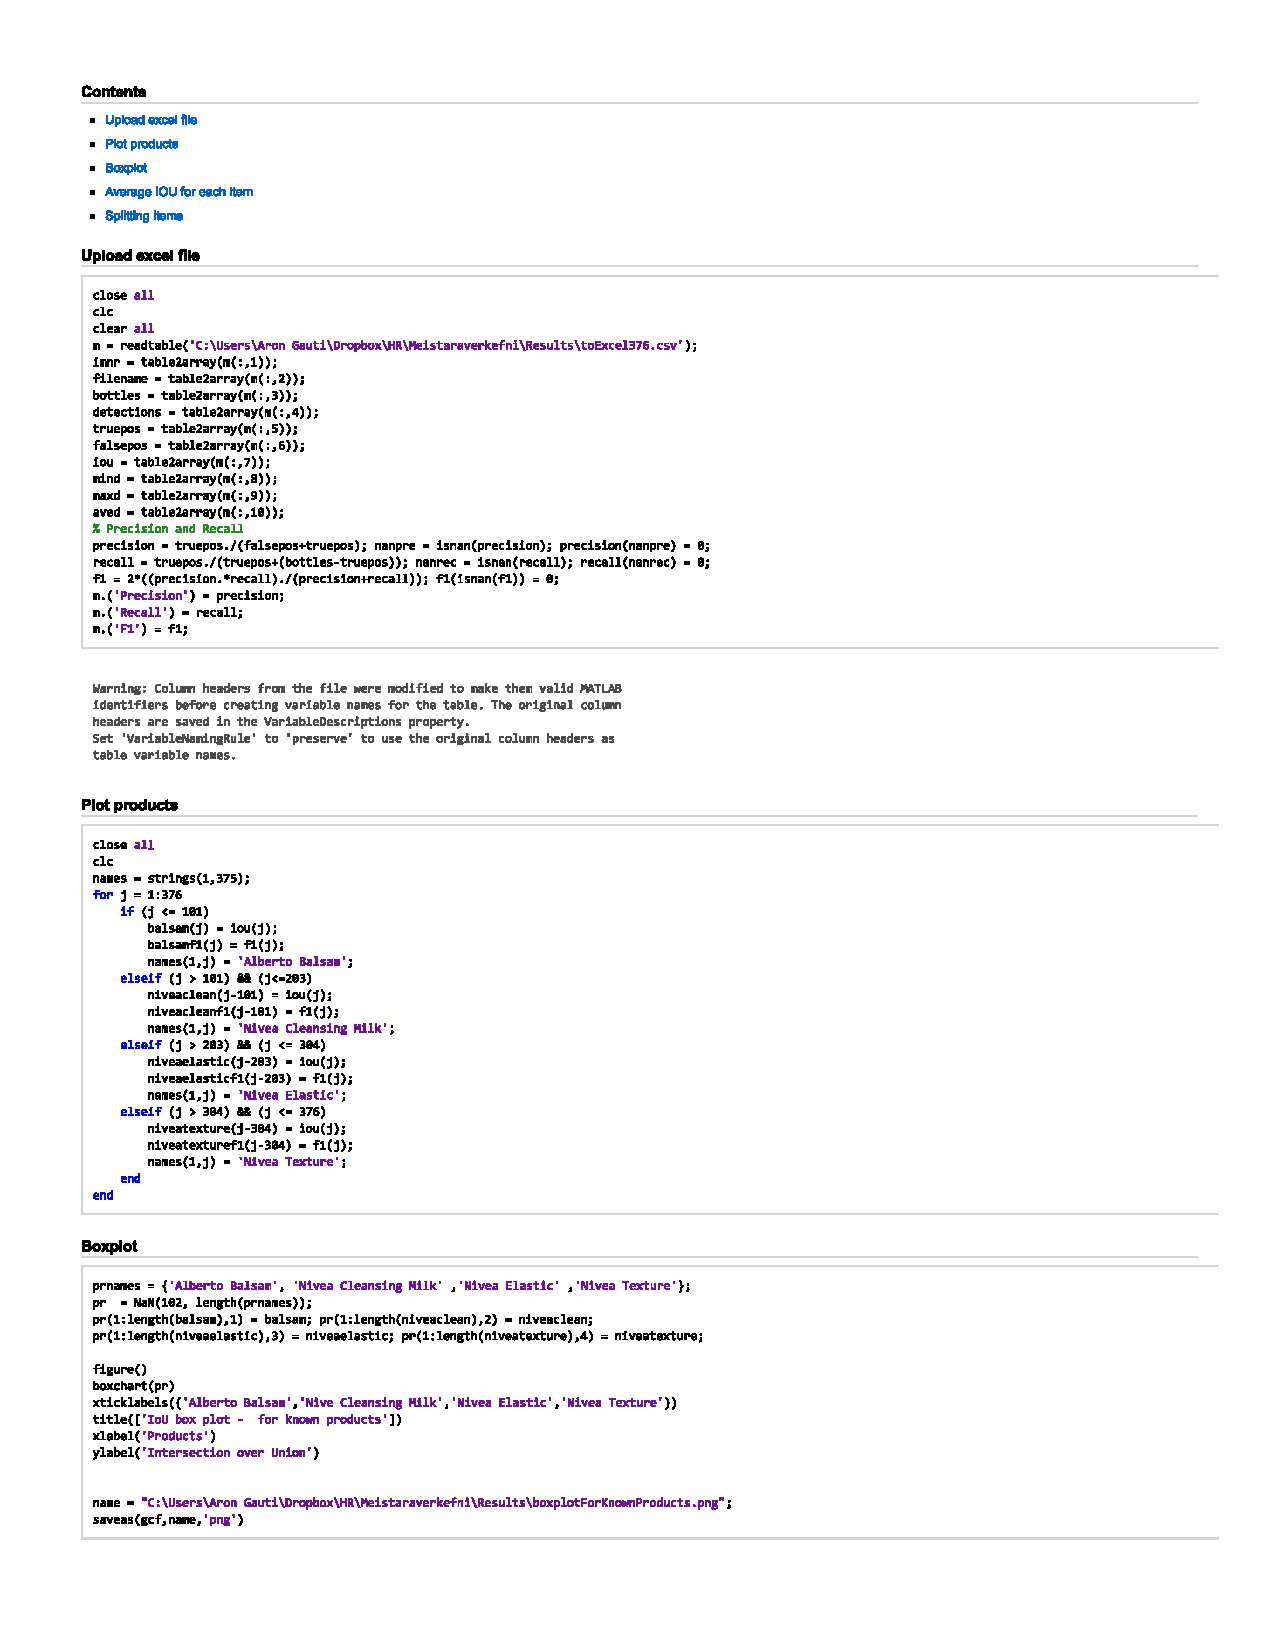
\includepdf[scale=0.8 ,pages=1, offset=0 -4cm]{appendix/knownitems.pdf}
\end{figure}
\includepdf[scale=1 ,pages={2,3,4,5}, offset=0 0cm]{appendix/knownitems.pdf}
\clearpage
\section{Results on unknown items}\label{sec:apIoUunknownresults}
\begin{figure}[h]
 \centering 
 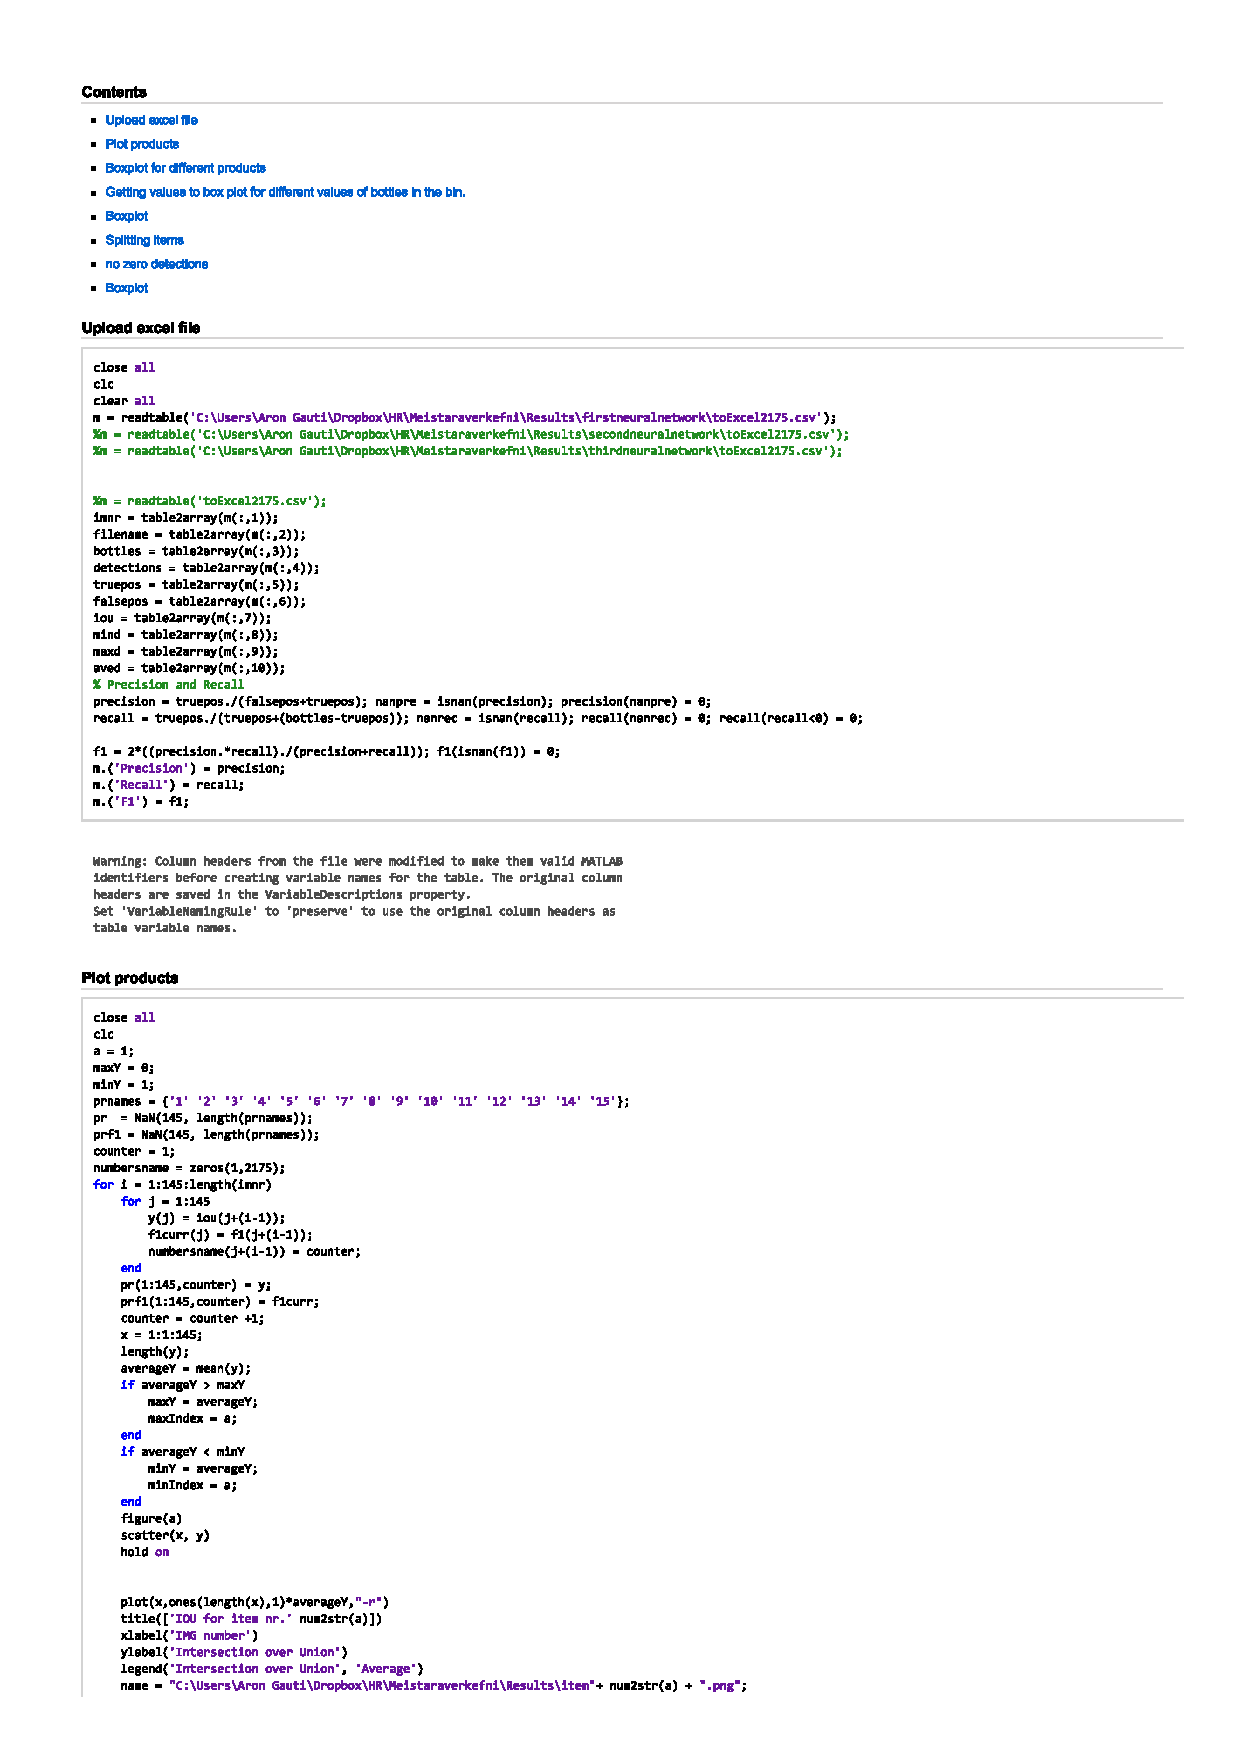
\includepdf[scale=0.98 ,pages=1, offset=0 -0.2cm]{appendix/unknownitems.pdf}
\end{figure}
\includepdf[scale=1 ,pages={2,3,4,5,6,7,8,9,10,11}, offset=0 0cm]{appendix/unknownitems.pdf}
\clearpage